\captionsetup{subrefformat=parens}

\label{apx:BlobToolsAnalysis}




\begin{figure}[hp!]
    \centering
    \begin{subfigure}[]{0.9\textwidth}
        \centering
        \includegraphics[width=\textwidth]{Appendices/S6_SPAdesAssembly-AllReads.blobtools.blobDB.json.bestsum.species.p8.span.100.blobplot.bam0.pdf}
        \caption{}
        \label{fig:BlobPlot-S6-All}
    \end{subfigure}
    \begin{subfigure}[]{0.9\textwidth}
        \centering
        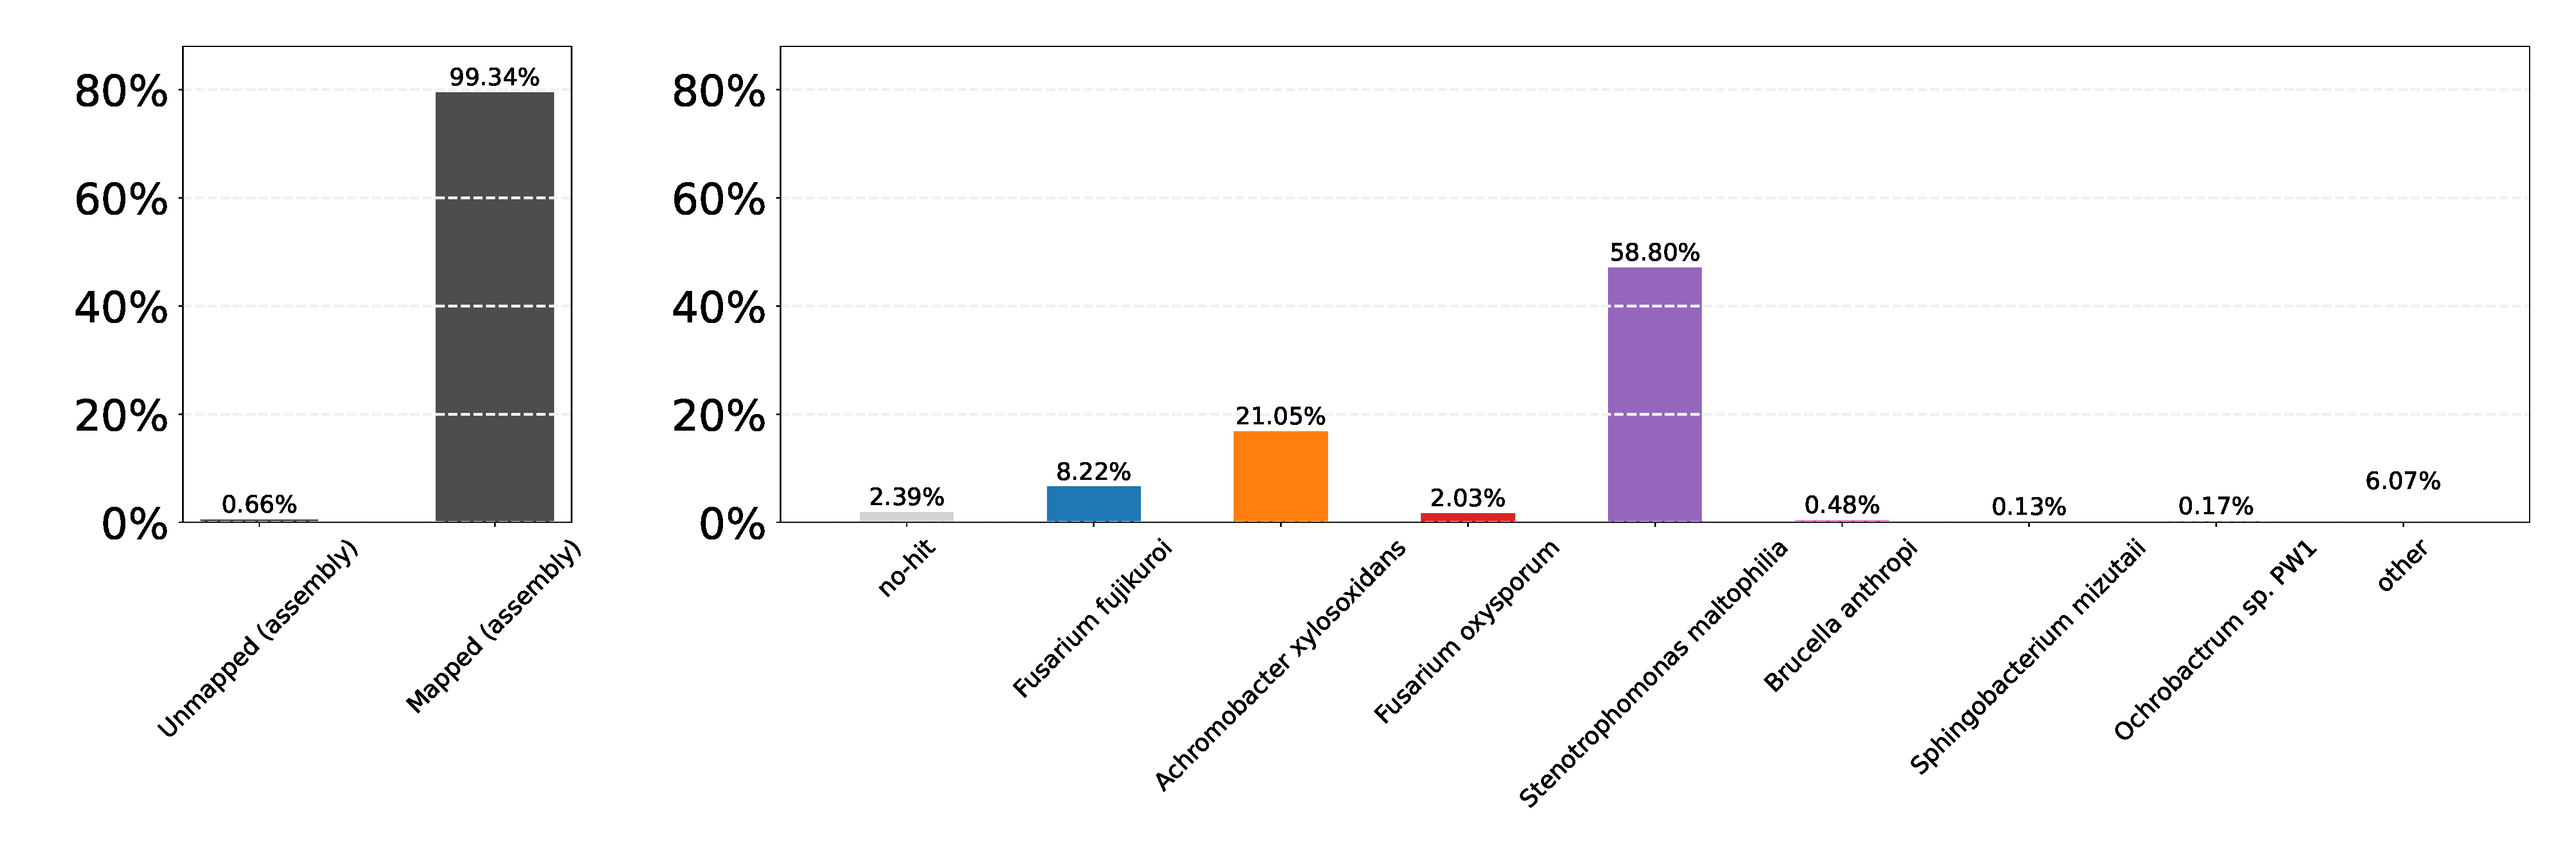
\includegraphics[width=\textwidth]{Appendices/S6_SPAdesAssembly-AllReads.blobtools.blobDB.json.bestsum.species.p8.span.100.blobplot.read_cov.bam0.pdf}
        \caption{}
        \label{fig:BlobPlot_readcov-S6-All}
    \end{subfigure}
    \caption[BlobTools visualisations of the unfiltered S6 assembly]{\textbf{BlobTools visualisations of the unfiltered S6 assembly shows bacterial contamination.}
        \subref{fig:BlobPlot-S6-All} BlobPlot of S6. Sequences in the unfiltered assembly are depicted as circles, with diameter proportional to sequence length and coloured by taxonomic annotation based on BLASTN (v2.9.0+) of NCBI nt database.
        \subref{fig:BlobPlot_readcov-S6-All} Read coverage plot of the unfiltered S6 assembly. Mapped reads are shown by taxonomic group at the rank of species.}
        \label{fig:S6:BlobToolsAllreads}
\end{figure}
\bigskip

\begin{figure}[hp!]
    \centering
    \begin{subfigure}[]{0.9\textwidth}
        \centering
        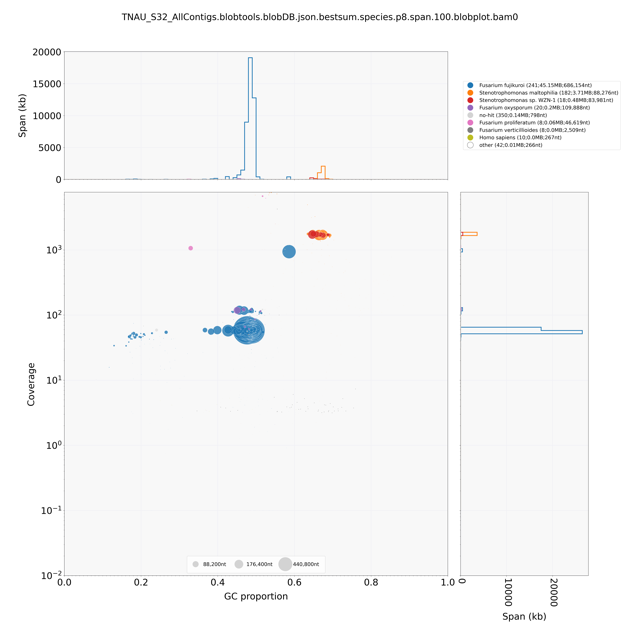
\includegraphics[width=\textwidth]{Figures/TNAU_S32_AllContigs.blobtools.blobDB.json.bestsum.species.p8.span.100.blobplot.bam0.png}
        \caption{}
        \label{fig:BlobPlot-S32-All}
    \end{subfigure}
    \begin{subfigure}[]{0.9\textwidth}
        \centering
        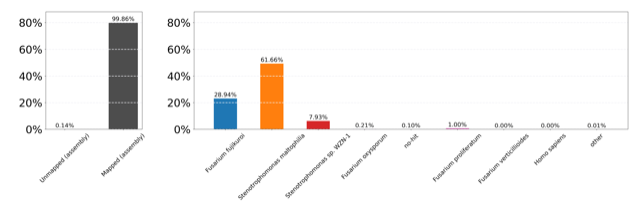
\includegraphics[width=\textwidth]{Figures/TNAU_S32_AllContigs.blobtools.blobDB.json.bestsum.species.p8.span.100.blobplot.read_cov.bam0.png}
        \caption{}
        \label{fig:BlobPlot_readcov-S32-All}
    \end{subfigure}
    \caption[BlobTools visualisations of the unfiltered S32 assembly]{\textbf{BlobTools visualisations of the unfiltered S32 assembly shows bacterial contamination.}
        \subref{fig:BlobPlot-S32-All} BlobPlot of S32. Sequences in the unfiltered assembly are depicted as circles, with diameter proportional to sequence length and coloured by taxonomic annotation based on BLASTN (v2.9.0+) of NCBI nt database.
        \subref{fig:BlobPlot_readcov-S32-All} Read coverage plot of the unfiltered S32 assembly. Mapped reads are shown by taxonomic group at the rank of species.}
        \label{fig:S32:BlobToolsAllreads}
\end{figure}
\bigskip

\subsubsection{\acf{rbp2} Phylogeny of \textit{Fusarium} assemblies}

\begin{figure}[htp!]
    \centering
    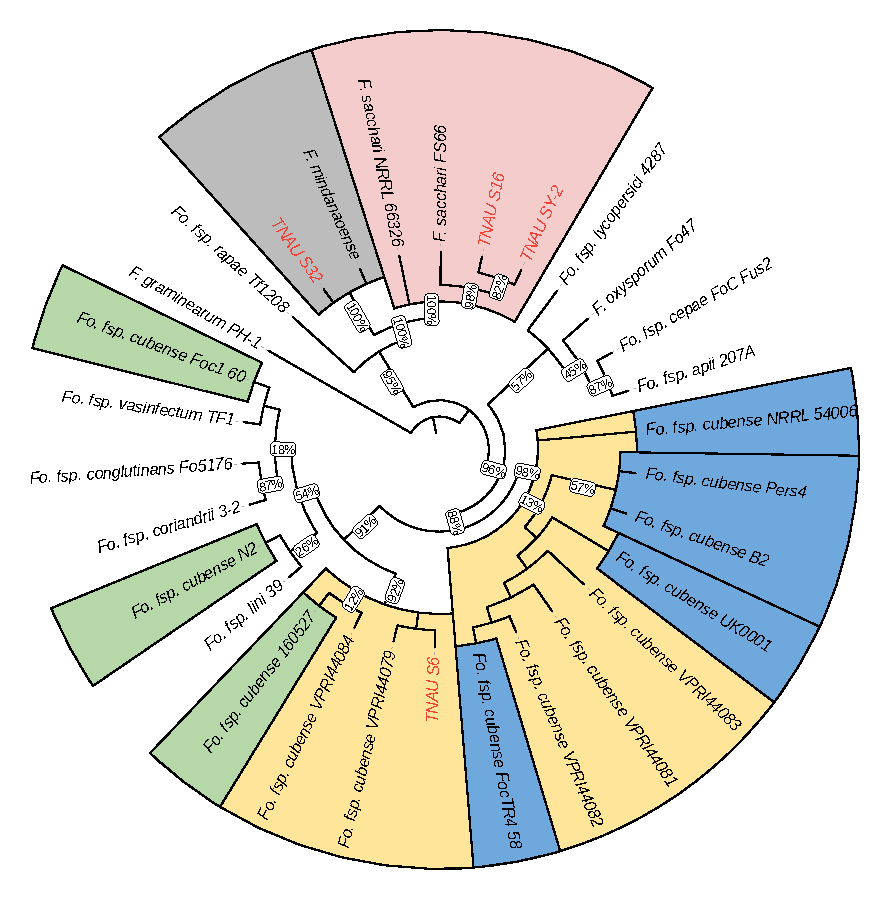
\includegraphics[width=14cm]{Appendices/RPNii-Phylogeny.pdf}
    \caption[\Acl{rbp2} phylogeny of \acl{tnau} \textit{Fusarium} isolates.]{\textbf{\Acl{rbp2} phylogeny of \acl{tnau} \textit{Fusarium} isolates.} \Ac{tnau} isolates S16, S32 and SY-2 sit within the \acf{FFSC} clade. The isolates from \ac{tnau} are shown in red text. The \acf{Fs} clade is shown in pink. \Acf{Focub4} isolates are in blue. \Acf{Focub1} isolates are shown in green. \acf{Focub} isolates with race not recorded are shown in yellow. Percentages represent values from 1000 bootstrap replicates. The tree is rooted through \textit{Fusarium graminearum} PH-1 \ac{rbp2}.}
    \label{fig:rbp2Phylo}
\end{figure}
\bigskip